% Use only LaTeX2e, calling the article.cls class and 12-point type.

\documentclass[12pt]{article}

%Cosas copiadas del paper de Iñigo
\usepackage[table]{xcolor}
\RequirePackage{siunitx}
\RequirePackage[T1]{fontenc}                        % T1 font encoding for PDFs
\RequirePackage{lmodern}                                % extended font definition
\RequirePackage{amsmath,amssymb,amsthm} % most important math stuff
\RequirePackage{a4wide}                                 % make better use of A4 paper
\RequirePackage{fancyhdr}                               % custom headers and footers
\RequirePackage{fncychap}                               % custom chapter titles
\RequirePackage{graphicx}                               % graphics
\RequirePackage{color}                                  % color
\RequirePackage{booktabs}                               % extra tabular commands
\RequirePackage[format=plain]{caption}  % improved caption format
\RequirePackage{nomencl}                                % cool nomenclature listing
\RequirePackage{makeidx}                                % create your index
\RequirePackage[printonlyused]{acronym}
\RequirePackage{ifthen}                                 % if-then commands (used in maketitle)
\RequirePackage{eso-pic}                                % picture in back/forground (used in cover)
\RequirePackage{relsize}                                % \textlarger, \textsmaller etc
%%
%%
%%%%%%%%%%%%%%%%%%%%%%%%%%%%%%%%%%%%%%%%%%%%%%%%%%%%%%%%%%%%
%%
%%  Set up Matlab and C++ Listings
%%  REQUIRES PACKAGE listings AND colortbl
%%
%%%%%%%%%%%%%%%%%%%%%%%%%%%%%%%%%%%%%%%%%%%%%%%%%%%%%%%%%%%%
%%
%%

\RequirePackage{listings}%

\usepackage[utf8]{inputenc}

\usepackage{pgf,tikz}

\usepackage{pgfgantt}

\usepackage{mathrsfs}

\usepackage{mathtools}

\usepackage{gensymb}

\usepackage{float}

\usepackage{needspace}

\usepackage{pgfplots}

\usepackage[nodayofweek,level]{datetime}

\usepackage{todonotes}

\usepackage{bm}

\usepackage{enumitem}

\usepackage{graphicx}

\usepackage{subcaption}

\usepackage{indentfirst}

\usepackage{multirow}

\usepackage{eurosym}

\usepackage{hhline}

\usepackage{esvect}


\usepackage{upgreek}
\usepackage{arydshln}
\usepackage{algorithm}
\usepackage[noend]{algpseudocode}

\usepackage[nameinlink,capitalise]{cleveref}

\usepackage{mathtools}
%%%%%%%%%%% COPYPASTEADO DE GITHUB
\usepackage{amsmath}
\usepackage{amssymb}

\usepackage{wrapfig}

%redefine vector and Real symbols for faster typing
\renewcommand{\vec}[1]{\bm{#1}}
\newcommand{\R}{\mathbb R}
\newcommand{\Z}{\mathbb Z}
\newcommand{\foralli}[1][]{\forall i \in \{1\dots n_{#1}\}}
\newcommand{\forallj}[1][]{\forall j \in \{1\dots n_{#1}\}}
\newcommand{\forallk}[1][]{\forall k \in \{1\dots n_{#1}\}}
\newcommand{\dd}[2]{\frac{\partial #1}{\partial #2}}
\newcommand{\dt}[1]{\frac{d #1}{d t}}
\newcommand{\torque}{\tau}
\newcommand{\w}{\dot\varphi}
\newcommand{\h}{\frac{1}{2}}
\newcommand{\pare}[1]{\left(#1\right)}
\newcommand{\brac}[1]{\left\{#1\right\}}

\newcommand{\mat}[2][b]{\begin{#1matrix}#2\end{#1matrix}}

%set spacing between rows in tables
\renewcommand{\arraystretch}{1.2}

\def\F{\vec F}
\def\Torque{\vec \Gamma}
\def\R{\vec R}

\def\q{\vec q}
\def\M{\vec M}
\def\I{\vec I}
\def\C{\vec C}
\def\mults{\vec \lambda}

%   Fin de la parte copypasteada
\graphicspath{ {images/} }

% Users of the {thebibliography} environment or BibTeX should use the
% scicite.sty package, downloadable from *Science* at
% www.sciencemag.org/about/authors/prep/TeX_help/ .
% This package should properly format in-text
% reference calls and reference-list numbers.

\usepackage{scicite}

% Use times if you have the font installed; otherwise, comment out the
% following line.

\usepackage{times}

% The preamble here sets up a lot of new/revised commands and
% environments.  It's annoying, but please do *not* try to strip these
% out into a separate .sty file (which could lead to the loss of some
% information when we convert the file to other formats).  Instead, keep
% them in the preamble of your main LaTeX source file.


% The following parameters seem to provide a reasonable page setup.

\topmargin 0.0cm
\oddsidemargin 0.2cm
\textwidth 16cm 
\textheight 21cm
\footskip 1.0cm


%The next command sets up an environment for the abstract to your paper.

\newenvironment{sciabstract}{%
\begin{quote} \bf}
{\end{quote}}


% If your reference list includes text notes as well as references,
% include the following line; otherwise, comment it out.

\renewcommand\refname{References and Notes}

% The following lines set up an environment for the last note in the
% reference list, which commonly includes acknowledgments of funding,
% help, etc.  It's intended for users of BibTeX or the {thebibliography}
% environment.  Users who are hand-coding their references at the end
% using a list environment such as {enumerate} can simply add another
% item at the end, and it will be numbered automatically.

\newcounter{lastnote}
\newenvironment{scilastnote}{%
\setcounter{lastnote}{\value{enumiv}}%
\addtocounter{lastnote}{+1}%
\begin{list}%
{\arabic{lastnote}.}
{\setlength{\leftmargin}{.22in}}
{\setlength{\labelsep}{.5em}}}
{\end{list}}


% Include your paper's title here

\title{Geometric considerations of an alternative axes for Omnibot} 


% Place the author information here.  Please hand-code the contact
% information and notecalls; do *not* use \footnote commands.  Let the
% author contact information appear immediately below the author names
% as shown.  We would also prefer that you don't change the type-size
% settings shown here.

\author
{Siro Moreno$^{1\ast}$ \\
\\
\normalsize{$^{1}$Institut de Robótica i Informática Industrial}\\
\normalsize{dirección del IRI, Barcelona}\\
\normalsize{$^\ast$To whom correspondence should be addressed; E-mail:  ejemplo@ejemplo.eje}
}

% Include the date command, but leave its argument blank.

\date{}



%%%%%%%%%%%%%%%%% END OF PREAMBLE %%%%%%%%%%%%%%%%



\begin{document} 

% Double-space the manuscript.

\baselineskip24pt

% Make the title.

\maketitle 



% Place your abstract within the special {sciabstract} environment.

\begin{sciabstract}
  We will discuss some considerations and insights of using an alternative axes with the Omnibot robot, rotated 45 degrees respect to the symmetry axes.
\end{sciabstract}



% In setting up this template for *Science* papers, we've used both
% the \section* command and the \paragraph* command for topical
% divisions.  Which you use will of course depend on the type of paper
% you're writing.  Review Articles tend to have displayed headings, for
% which \section* is more appropriate; Research Articles, when they have
% formal topical divisions at all, tend to signal them with bold text
% that runs into the paragraph, for which \paragraph* is the right
% choice.  Either way, use the asterisk (*) modifier, as shown, to
% suppress numbering.

\section*{Definition of new axes}

\begin{wrapfigure}{l}{0.3\textwidth}
	\centering
	\includegraphics[width=\linewidth]{Omnibot_45_deg.png}
	\captionof{figure}{Omnibot new axes}
	\label{fig:omnibot}
\end{wrapfigure}
Let's define a new vector base system, anchored to the center of mass of the Omnibot and rotated 45 degrees clockwise respect to the B basis.
In order to describe the position of the wheels in this new base, we can define the magnitudes:
$$ l_2 = \frac{L-l}{\sqrt{2}}\ , \ L_2 = \frac{L+l}{\sqrt{2}}$$
We can follow the same process to calculate the equations of the system, but using the base 2 instead of the base B as an intermediate base between the $q_r$ and $q_w$ coordinates. We will also define $psi$ as the angle between the global X axis and the $x_2$ axis, instead of using the $x_B$ axis.

The first difference that we can observe is that using this base, some zeroes appear on the R matrix:

$$ R = \frac{\sqrt{2}}{r}\left[\begin{matrix}1 & 0 & - L_{2}\\0 & 1 & L_{2}\\0 & 1 & - L_{2}\\1 & 0 & L_{2}\end{matrix}\right]$$

We observe that movement on $x_2$ and $y_2$ uncouples.

\subsection*{Definition of $\dot{\q}_2$ and $\ddot{\q}_2$ }

Let's define two new concepts: $\dot{\q}_2$ and $\ddot{\q}_2$:

$$ \dot{\q}_2 \equiv \left[\begin{matrix}\dot{x}_{2}\\\dot{y}_{2}\\\dot{\psi}\end{matrix}\right] = \R_{\psi}^T \dot{\q_r}\ ,\ \ddot{\q}_2 \equiv \left[\begin{matrix}\ddot{x}_{2}\\\ddot{y}_{2}\\\ddot{\psi}\end{matrix}\right] = \R_{\psi}^T \ddot{\q_r}$$

We observe that $\dot{\q}_2$ and $\ddot{\q}_2$ are the proyection on base 2 of the global speeds and accelerations. We must be cautious when using them, because since $\R_{\psi}$ can vary with time, in general $\frac{d\dot{\q}_2}{dt}\neq\ddot{\q}_2$.
$$\frac{d\dot{\q}_2}{dt} = \frac{d(\R_{\psi}^T \dot{\q_r})}{dt} =  \frac{d(\R_{\psi}^T)}{dt}\dot{\q_r} + \R_{\psi}^T \ddot{\q_r}=  \frac{d(\R_{\psi}^T)}{dt}\dot{\q_r} + \ddot{\q_2}$$

Why are then these variables useful? The answer begins with the relationship that connects $\dot{\q_r}$ and $\dot{\q_w}$:
$$\dot{\q_w} = \R \R_{\psi}^T \dot{\q_r} = \R \dot{\q_2} = \frac{\sqrt{2}}{2}\left[\begin{matrix}- L_{2} \dot{\psi} + \dot{x}_{2}\\L_{2} \dot{\psi} + \dot{y}_{2}\\- L_{2} \dot{\psi} + \dot{y}_{2}\\L_{2} \dot{\psi} + \dot{x}_{2}\end{matrix}\right]$$
We can observe from this that rotation of wheels 1 and 4 only depend on $\dot{\psi}$ and $\dot{x_2}$, while rotation of wheels 2 and 3 only depend on $\dot{\psi}$ and $\dot{y_2}$.

This means that, as the speed of the robot is limited by the maximum speed in any of its wheels' shafts, the envelope of achievable speeds in $x_2$ and $y_2$ will always be a square whose size depends on $\dot{\psi}$:
\begin{figure}[h]
	\centering
	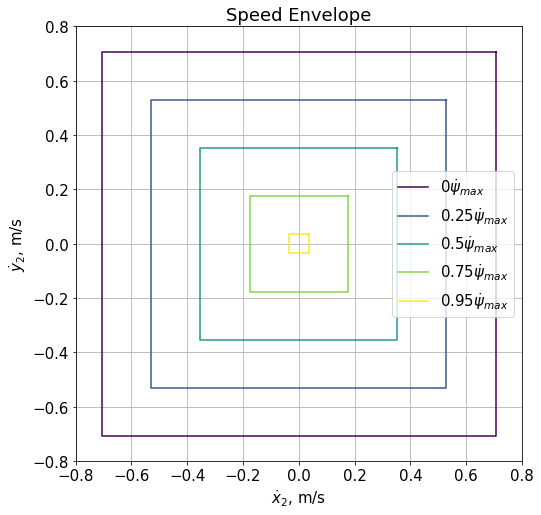
\includegraphics[width=.5\linewidth]{speed_envelope}
	\captionof{figure}{Speed Envelope}
	\label{fig:speed_envelope}
\end{figure}

\section*{Proyection of the equation}

As we know from the work of Iñigo, we can describe the Omnibot system dynamics as
\begin{gather}
	\underbrace{(\M_r+\R_{\psi}\R ^T
		\M_w\R \R_{\psi}^T)}_{\vec H}\ddot \q_r+
	\underbrace{\R_{\psi}\R ^T\M_w\R \dot{\R}_{\psi}^T}_{\vec K}\dot \q_r=\R_{\psi}\R ^T\Torque \label{eq:solution}
\end{gather}
Where:
\begin{gather}
	\vec H = \mat{ m+\frac{4\,I_w}{r^2} & 0 & 0 \\ 0 & m+\frac{4\,I_w}{r^2} & 0 \\ 0 & 0 & I_z+\frac{4\,I_w\,{\left(L+l\right)}^2}{r^2} } \label{eq:H}
	\\
	\vec K = \mat{ 0 & \frac{4\,I_w\,\dot \psi }{r^2} & 0 \\ -\frac{4\,I_w\,\dot \psi }{r^2} & 0 & 0 \\ 0 & 0 & 0 }
\end{gather}

Now, let's assume that the robot is moving with constant speed in a direction defined by the  $\gamma$ angle, without rotating:


Let's also assume that $\psi$ is zero for simplicity, so the robot is facing the global X axis.

Since $\ddot{\q_r} = 0$ and $\dot{\psi} = 0$, we can see that $\Torque$ must be zero as well. This means that if we don't consider frictions outside the motors, no torque is required to keep the uniform movement. Since the mechanical power produced by the wheel axes are their torques times their speeds, we can see that they provide no power. As expected, in absence of friction, no energy needs to be expended in order to keep a straight uniform movement.

We can get more insight from this configuration. We know that $\dot{\q_w} = \R \R_{\psi}^T \dot{\q_r}$, so we can observe how the wheels move in this situation. We will use a speed value of 1 m/s for this example.
\begin{figure}[h]
	\centering
	\begin{minipage}{.5\textwidth}
		\centering
		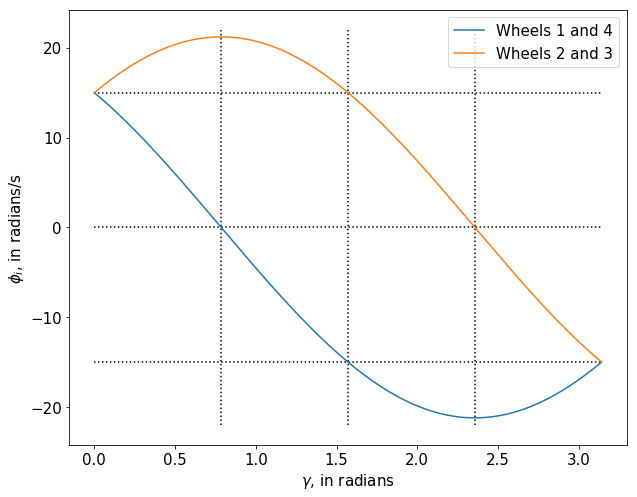
\includegraphics[width=.9\linewidth]{wheel_speeds}
		\captionof{figure}{Speed of wheels}
		\label{fig:wheel_speed}
	\end{minipage}%
	\begin{minipage}{.5\textwidth}
		\centering
		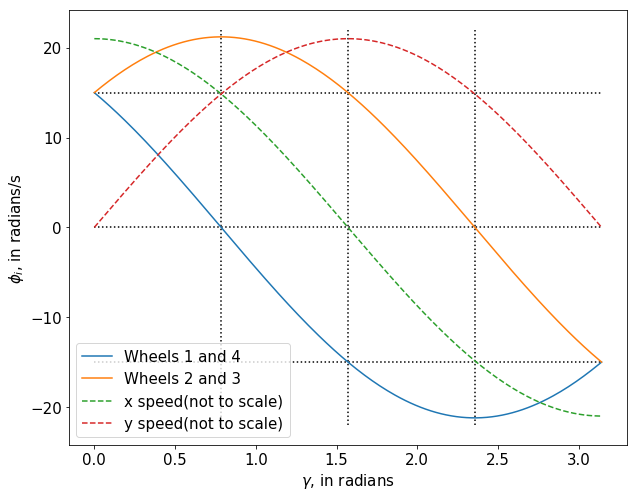
\includegraphics[width=.9\linewidth]{wheel_xy_speeds}
		\captionof{figure}{Speed of wheels with reference}
		\label{fig:wheel_speed_xy}
	\end{minipage}
\end{figure}
When we compare the speed of the wheels with the components in x and y of the velocity, we can imagine that it could be an interesting exercise to turn the robot axes 45 degrees respect to the current chassis configuration. Later we will use the absolute value of wheel speeds, so we can also plot them here for reference:
\begin{figure}[h]
	\centering
	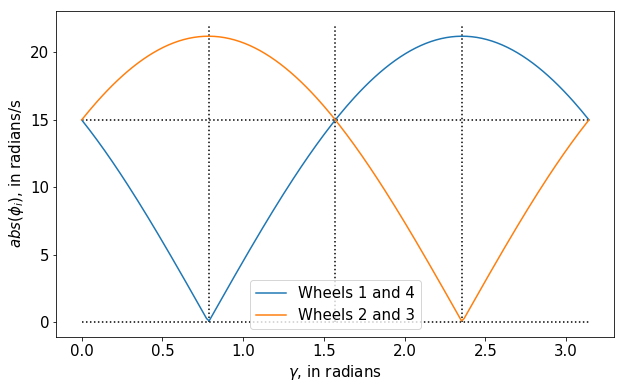
\includegraphics[width=.5\linewidth]{abs_wheel_speeds}
	\captionof{figure}{Absolute speed of wheels}
	\label{fig:abs_wheel_speed}
\end{figure}

Lets assume again that we are moving in a direction defined by angle $\gamma$, with $\psi = 0$ and not rotating, but now with constant speed $v_r$ .
$$\dot{\q_r} = v_r\left[\begin{matrix}\operatorname{cos}\left(\gamma\right)\\\operatorname{sin}\left(\gamma\right)\\0\end{matrix}\right]\ ,\ \psi = \dot{\psi} = 0\ ,\ \Torque = \ddot{\q_r} = \vec{0}$$
$$ \dot{\q_w} = \R\R_{\psi}^T\dot{\q_r} = \left[\begin{matrix}\frac{\sqrt{2} v_{r} \operatorname{cos}\left(\gamma + \frac{\pi}{4}\right)}{r}\\\frac{\sqrt{2} v_{r} \operatorname{sin}\left(\gamma + \frac{\pi}{4}\right)}{r}\\\frac{\sqrt{2} v_{r} \operatorname{sin}\left(\gamma + \frac{\pi}{4}\right)}{r}\\\frac{\sqrt{2} v_{r} \operatorname{cos}\left(\gamma + \frac{\pi}{4}\right)}{r}\end{matrix}\right]$$

We know, from the manufacturer and experiments, that the maximum speed of any motor at maximum voltage is 14.96 rads/s.We can see that for gamma between 0 and pi/2, wheels 2 and 3 are the limit. Between pi/2 and pi, wheels 1 and 4 are the limit. We can then plot the maximum $v_r$ achievable as a function of $\gamma$:

\begin{figure}[h]
	\centering
	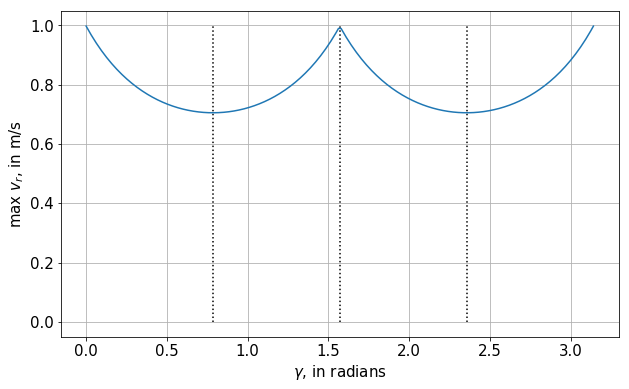
\includegraphics[width=.5\linewidth]{max_vr_gamma}
	\captionof{figure}{Max speed in gamma}
	\label{fig:max_vr_gamma}
\end{figure}
We can confirm that the maximum speed depends on the direction, and observe that the maximum speed is largest when it is parallel to the X or Y axes.

\section*{Accelerated movement}

Lets work now with an accelerated movement, in a consant direction defined by the angle $\gamma$, with no rotation. The speed is $v(t)$ and the acceleration is $a(t) = \dot{v}(t)$.
$$\ddot{\q_r} = \left[\begin{matrix}a \operatorname{cos}\left(\gamma\right)\\a \operatorname{sin}\left(\gamma\right)\\0\end{matrix}\right],
\dot{\q_r} =  \left[\begin{matrix}v \operatorname{cos}\left(\gamma\right)\\v \operatorname{sin}\left(\gamma\right)\\0\end{matrix}\right], \psi = \dot{\psi} = 0$$
$$\vec H \ddot{\q_r} = \R^T \Torque$$

By multiplying both sides of the equation by the pseudoinverse $R^-1$, we get the Torque array that does not have components in the kernel direction, that is, that doesn't contribute to the movement.

$$ \R^{-1T} \vec H \ddot{\q_r} =\Torque$$

Operating, we get: 
$$\Torque = \left[\begin{matrix}\frac{\sqrt{2} \left(4 I_{w} + m r^{2}\right) a \operatorname{cos}\left(\gamma + \frac{\pi}{4}\right)}{4 r}\\\frac{\sqrt{2} \left(4 I_{w} + m r^{2}\right) a \operatorname{sin}\left(\gamma + \frac{\pi}{4}\right)}{4 r}\\\frac{\sqrt{2} \left(4 I_{w} + m r^{2}\right) a \operatorname{sin}\left(\gamma + \frac{\pi}{4}\right)}{4 r}\\\frac{\sqrt{2} \left(4 I_{w} + m r^{2}\right) a \operatorname{cos}\left(\gamma + \frac{\pi}{4}\right)}{4 r}\end{matrix}\right] ,
 \dot{\q_w} =  \left[\begin{matrix}- \frac{v \operatorname{sin}\left(\gamma\right)}{r} + \frac{v \operatorname{cos}\left(\gamma\right)}{r}\\\frac{v \operatorname{sin}\left(\gamma\right)}{r} + \frac{v \operatorname{cos}\left(\gamma\right)}{r}\\\frac{v \operatorname{sin}\left(\gamma\right)}{r} + \frac{v \operatorname{cos}\left(\gamma\right)}{r}\\- \frac{v \operatorname{sin}\left(\gamma\right)}{r} + \frac{v \operatorname{cos}\left(\gamma\right)}{r}\end{matrix}\right]$$

And since the mechanical power exerted by the wheel axes are $\Torque  \dot{\q_w}$, operating we finally obtain:
$$ P_{mec} =\frac{\left(4 I_{w} + m r^{2}\right) a v}{r^{2}} =\frac{\left(4 I_{w} + m r^{2}\right) \dot{v} v}{r^{2}}$$

If we integrate the power for $t$, we get the energy produced by the wheels axes:

$$E_{mec} = \frac{2 I_{w} v^{2}}{r^{2}} + \frac{m v^{2}}{2}$$

Which we can observe that is exactly the kinetic energy of the robot. We can also oberve that, even if the movement of the wheels depend on the direction, due to the geometry of the robot, the total kinetic energy does not. 

\subsection*{General case}

We can take a step further and consider a completely general case:
$$\ddot{\q_r} = \left[\begin{matrix}\ddot{x}\\\ddot{y}\\\ddot{\psi}\end{matrix}\right], \ \dot{\q_r} \left[\begin{matrix}\dot{x}\\\dot{y}\\\dot{\psi}\end{matrix}\right]$$

Again:

$$ \R^{-1T} \vec H \ddot{\q_r} =\Torque$$

Operating, we get: 
$$\Torque = \left[\begin{matrix}\frac{\sqrt{2} \left(4 I_{w} + m r^{2}\right) \left(L + l\right) \left(\operatorname{sin}\left(\psi + \frac{\pi}{4}\right) \ddot{x} - \operatorname{cos}\left(\psi + \frac{\pi}{4}\right) \ddot{y}\right) - \left(4 I_{w} \left(L + l\right)^{2} + I_{z} r^{2}\right) \ddot{\psi}}{4 r \left(L + l\right)}\\\frac{\sqrt{2} \left(4 I_{w} + m r^{2}\right) \left(L + l\right) \left(\operatorname{sin}\left(\psi + \frac{\pi}{4}\right) \ddot{y} + \operatorname{cos}\left(\psi + \frac{\pi}{4}\right) \ddot{x}\right) + \left(4 I_{w} \left(L + l\right)^{2} + I_{z} r^{2}\right) \ddot{\psi}}{4 r \left(L + l\right)}\\\frac{\sqrt{2} \left(4 I_{w} + m r^{2}\right) \left(L + l\right) \left(\operatorname{sin}\left(\psi + \frac{\pi}{4}\right) \ddot{y} + \operatorname{cos}\left(\psi + \frac{\pi}{4}\right) \ddot{x}\right) - \left(4 I_{w} \left(L + l\right)^{2} + I_{z} r^{2}\right) \ddot{\psi}}{4 r \left(L + l\right)}\\\frac{\sqrt{2} \left(4 I_{w} + m r^{2}\right) \left(L + l\right) \left(\operatorname{sin}\left(\psi + \frac{\pi}{4}\right) \ddot{x} - \operatorname{cos}\left(\psi + \frac{\pi}{4}\right) \ddot{y}\right) + \left(4 I_{w} \left(L + l\right)^{2} + I_{z} r^{2}\right) \ddot{\psi}}{4 r \left(L + l\right)}\end{matrix}\right] $$
$$\dot{\q_w} =   \left[\begin{matrix}\left(\frac{\operatorname{sin}\left(\psi\right)}{r} - \frac{\operatorname{cos}\left(\psi\right)}{r}\right) \dot{y} + \left(\frac{\operatorname{sin}\left(\psi\right)}{r} + \frac{\operatorname{cos}\left(\psi\right)}{r}\right) \dot{x} + \frac{\left(- L - l\right) \dot{\psi}}{r}\\\left(- \frac{\operatorname{sin}\left(\psi\right)}{r} + \frac{\operatorname{cos}\left(\psi\right)}{r}\right) \dot{x} + \left(\frac{\operatorname{sin}\left(\psi\right)}{r} + \frac{\operatorname{cos}\left(\psi\right)}{r}\right) \dot{y} + \frac{\left(L + l\right) \dot{\psi}}{r}\\\left(- \frac{\operatorname{sin}\left(\psi\right)}{r} + \frac{\operatorname{cos}\left(\psi\right)}{r}\right) \dot{x} + \left(\frac{\operatorname{sin}\left(\psi\right)}{r} + \frac{\operatorname{cos}\left(\psi\right)}{r}\right) \dot{y} + \frac{\left(- L - l\right) \dot{\psi}}{r}\\\left(\frac{\operatorname{sin}\left(\psi\right)}{r} - \frac{\operatorname{cos}\left(\psi\right)}{r}\right) \dot{y} + \left(\frac{\operatorname{sin}\left(\psi\right)}{r} + \frac{\operatorname{cos}\left(\psi\right)}{r}\right) \dot{x} + \frac{\left(L + l\right) \dot{\psi}}{r}\end{matrix}\right]$$

Operating we finally get:
$$ P_{mec} = \left[\begin{matrix}\frac{4 I_{w} L^{2} \dot{\psi} \ddot{\psi} + 8 I_{w} L l \dot{\psi} \ddot{\psi} + 4 I_{w} l^{2} \dot{\psi} \ddot{\psi} + 4 I_{w} \dot{x} \ddot{x} + 4 I_{w} \dot{y} \ddot{y} + I_{z} r^{2} \dot{\psi} \ddot{\psi} + m r^{2} \dot{x} \ddot{x} + m r^{2} \dot{y} \ddot{y}}{r^{2}}\end{matrix}\right]$$

If we integrate the power for $t$, we get the energy produced by the wheels axes:

$$E_{mec} = \left[\begin{matrix}\frac{2 I_{w} L^{2} \dot{\psi}^{2}}{r^{2}} + \frac{4 I_{w} L l \dot{\psi}^{2}}{r^{2}} + \frac{2 I_{w} l^{2} \dot{\psi}^{2}}{r^{2}} + \frac{2 I_{w} \dot{x}^{2}}{r^{2}} + \frac{2 I_{w} \dot{y}^{2}}{r^{2}} + \frac{I_{z} \dot{\psi}^{2}}{2} + \frac{m \dot{x}^{2}}{2} + \frac{m \dot{y}^{2}}{2}\end{matrix}\right]$$

Which we can observe that still is exactly the kinetic energy of the robot. We can also oberve that, even in this most general case, the total kinetic energy does not depend on the direction of the movenemt, as every instance of $\dot{x}$ and $\dot{y}$ can be simplified to the module of the velocity through $\dot{x}^2 + \dot{y}^2 = v^2$ and there are no terms dependant on $\psi$.
$$E_{mec} = \left[\begin{matrix}\frac{2 I_{w} L^{2} \dot{\psi}^{2}}{r^{2}} + \frac{4 I_{w} L l \dot{\psi}^{2}}{r^{2}} + \frac{2 I_{w} l^{2} \dot{\psi}^{2}}{r^{2}} + \frac{2 I_{w} v^{2}}{r^{2}} + \frac{I_{z} \dot{\psi}^{2}}{2} + \frac{m v^{2}}{2}\end{matrix}\right]$$

 This result confirms that, in absence of friction, all of the energy provided by the wheels axes converts into kinetic energy.
 
\section*{Electric Energy considerations}

Lets consider a motorreductor model based on Iñigo's but slightly more detailed:
$$ V = K_m \dot{\phi_{mot}} + Ri $$
$$ \tau_i = N K_ei \mu_{trans} - \tau_r $$
$$ \dot{\phi}_{mot} = N \dot{\phi}\ , \ \tau_r = a \dot{\phi} + b\ sign(\dot{\phi}) $$
Lets assume again that we are moving with constant speed $v_r$ in a direction defined by angle $\gamma$, with $\psi = 0$ and not rotating.
We know that $\tau_i = 0$, so we can express V and i as functions of $\phi$:
$$ i = \frac{1}{N K_e \mu}(a \dot{\phi} + b\ sign(\dot{\phi}) )$$
$$ V =  K_m N \dot{\phi} + Ri = K_m N \dot{\phi} +\frac{R}{N K_e \mu}(a \dot{\phi} + b\ sign(\dot{\phi}) )$$
Knowing that the electric power i $V i$:
$$ P_e = \left(\frac{K_{m} a}{K_{e} \mu} + \frac{R_{e} a^{2}}{K_{e}^{2} \mu^{2} n^{2}}\right) \dot{\phi}^{2} + \left(\frac{K_{m} b \operatorname{sign}\left(\dot{\phi}\right)}{K_{e} \mu} + \frac{2 R_{e} a b \operatorname{sign}\left(\dot{\phi}\right)}{K_{e}^{2} \mu^{2} n^{2}}\right) \dot{\phi} + \frac{R_{e} b^{2} \operatorname{sign}^{2}\left(\dot{\phi}\right)}{K_{e}^{2} \mu^{2} n^{2}}$$

If we substitute the values of the parameters, and plot the results in the range of feasible values, we can get a better understanding:
$$ P_e = 0.301 \operatorname{sign}^{2}\left(\dot{\phi}\right) + 0.638 \operatorname{sign}\left(\dot{\phi}\right) \dot{\phi} + 0.016 \dot{\phi}^{2}$$
\begin{figure}[h]
	\centering
	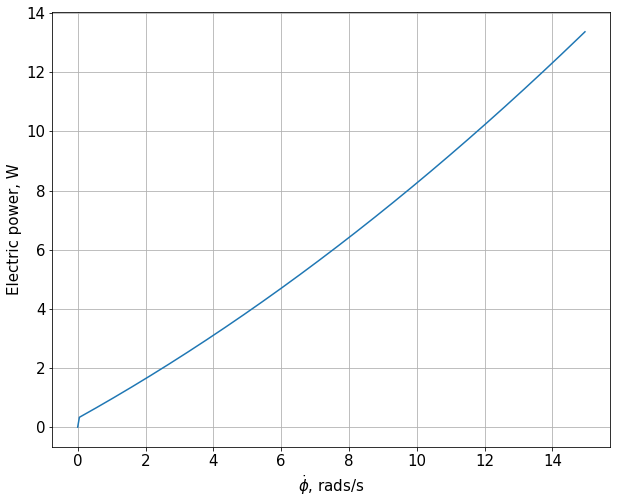
\includegraphics[width=.5\linewidth]{pe_phidot}
	\captionof{figure}{Electric power consumed}
	\label{fig:pe_phidot}
\end{figure}

We know the speeds:
$$\dot{\q_r} = v_r\left[\begin{matrix}\operatorname{cos}\left(\gamma\right)\\\operatorname{sin}\left(\gamma\right)\\0\end{matrix}\right]\ ,\ \psi = \dot{\psi} = 0\ ,\ \Torque = \ddot{\q_r} = \vec{0}$$
$$ \dot{\q_w} = \R\R_{\psi}^T\dot{\q_r} = \left[\begin{matrix}\frac{\sqrt{2} v_{r} \operatorname{cos}\left(\gamma + \frac{\pi}{4}\right)}{r}\\\frac{\sqrt{2} v_{r} \operatorname{sin}\left(\gamma + \frac{\pi}{4}\right)}{r}\\\frac{\sqrt{2} v_{r} \operatorname{sin}\left(\gamma + \frac{\pi}{4}\right)}{r}\\\frac{\sqrt{2} v_{r} \operatorname{cos}\left(\gamma + \frac{\pi}{4}\right)}{r}\end{matrix}\right]$$


The total power consumed is the sum of the power of the four motors. Substituting the value of the wheel radius for clarity, we can represent total power consumption as a function of $v_r$ and $\gamma$:
$$P_{e,tot} =14.17 v_{r}^{2} + 27.05 v_{r} \operatorname{sin}\left(\gamma + \frac{\pi}{4}\right) \operatorname{sign}\left(v_{r} \operatorname{sin}\left(\gamma + \frac{\pi}{4}\right)\right) +$$
$$+ 27.05 v_{r} \operatorname{cos}\left(\gamma + \frac{\pi}{4}\right) \operatorname{sign}\left(v_{r} \operatorname{cos}\left(\gamma + \frac{\pi}{4}\right)\right) +$$ 
$$+ 0.6 \operatorname{sign}^{2}\left(v_{r} \operatorname{sin}\left(\gamma + \frac{\pi}{4}\right)\right) + 0.6 \operatorname{sign}^{2}\left(v_{r} \operatorname{cos}\left(\gamma + \frac{\pi}{4}\right)\right)$$
If we consider $v_{r,max}$ the maximum speed achievable in the most unfavourable direction (45 degrees):
\begin{figure}[h]
	\centering
	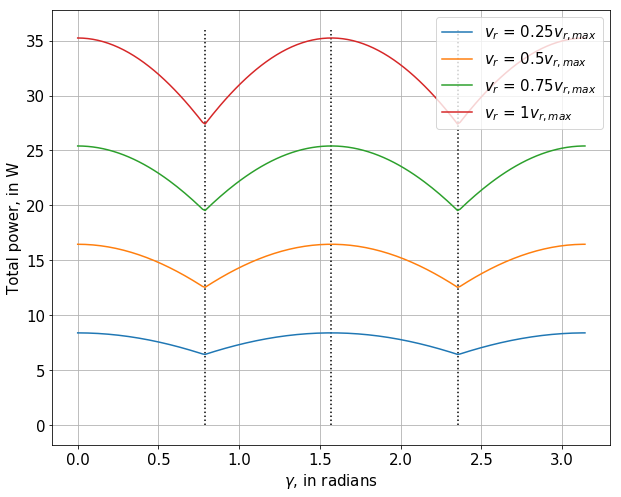
\includegraphics[width=.5\linewidth]{total_power}
	\captionof{figure}{Total electric power consumed}
	\label{fig:total_power}
\end{figure}

\section*{Conclusions}

We can reach maximum speed in directions parallel to the $X_{body}$ and $Y_{body}$ axes.

If we consider only the mechanical model without friction or the motors, all the energy output of the shafts are converted into kinetic energy, with independence of the advence direction.

If we consider also the motors, directions parallel to the body axes require more power than those at 45 degrees.
% Your references go at the end of the main text, and before the
% figures.  For this document we've used BibTeX, the .bib file
% scibib.bib, and the .bst file Science.bst.  The package scicite.sty
% was included to format the reference numbers according to *Science*
% style.


%\bibliography{scibib}

%\bibliographystyle{Science}



% Following is a new environment, {scilastnote}, that's defined in the
% preamble and that allows authors to add a reference at the end of the
% list that's not signaled in the text; such references are used in
% *Science* for acknowledgments of funding, help, etc.

%\begin{scilastnote}
%\item We've included in the template file \texttt{scifile.tex} a new
%environment, \texttt{\{scilastnote\}}, that generates a numbered final
%citation without a corresponding signal in the text.  This environment
%can be used to generate a final numbered reference containing
%acknowledgments, sources of funding, and the like, per {\it Science\/}
%style.
%\end{scilastnote}




% For your review copy (i.e., the file you initially send in for
% evaluation), you can use the {figure} environment and the
% \includegraphics command to stream your figures into the text, placing
% all figures at the end.  For the final, revised manuscript for
% acceptance and production, however, PostScript or other graphics
% should not be streamed into your compliled file.  Instead, set
% captions as simple paragraphs (with a \noindent tag), setting them
% off from the rest of the text with a \clearpage as shown  below, and
% submit figures as separate files according to the Art Department's
% instructions.


%\clearpage

%\noindent {\bf Fig. 1.} Please do not use figure environments to set
%up your figures in the final (post-peer-review) draft, do not include graphics in your
%source code, and do not cite figures in the text using \LaTeX\
%\verb+\ref+ commands.  Instead, simply refer to the figure numbers in
%the text per {\it Science\/} style, and include the list of captions at
%the end of the document, coded as ordinary paragraphs as shown in the
%\texttt{scifile.tex} template file.  Your actual figure files should
%be submitted separately.



\end{document}




















